\subsection{Parking Lot Generation}
The ParkingGenerator is responsible for filling roughly ten percent of the generated world's plots with parking lots.
This is based on research conducted in the city of Phoenix, Arizona \cite{percent}.
The ParkingGenerator is implemented as a function that takes a plot and its underlying terrain as input and produces a parking lot as output (see Table~\ref{table:parking}.
\begin{table}[H]
   \centering
   \begin{tabular}{lllll}
     \textbf{Input}                           &               & \textbf{Function}            &               & \textbf{Output}         \\
     \midrule
     \textit{Plot, Terrain}                   & $\rightarrow$ & \textbf{ParkingGenerator}       & $\rightarrow$ & \textit{Parking lot}           \\
     \bottomrule
   \end{tabular}

   \caption{Definition of the ParkingGenerator function which is responsible for generating parking lots.}
   \label{table:parking}
 \end{table}
 \vspace{-0.4cm}


One approach for generating parking lots for could have been using Esri CityEngine's \cite{Esri} one. % having a hard time finding this source, Anton who found it... plz help me. 
What they use for some of their generation is simply filling areas with textures, this is used for their parks as well as their parking lots. 
So for an example, their plots designated to be parking lots would simply be painted over with a \textit{parking-lot} texture. 
This was at first considered to be a viable option for the project, only it offers little alternatives for modification. 
Modification including shapes of the full parking lot as well as the size of the individual parking spaces. 
As every other generator provides content that is fully scalable it would be inconvenient to make use of a texture that could not be rescaled as easily, if at all.

The approach instead elected for was an algorithm that generates the parking spaces individually.
This algorithm works by first using a function for approximating the largest rectangle inside any given polygon. 
The reasoning behind this was the group's observation that a lot of parking lots seem to be shaped in rectangular ways (see Figure~\ref{fig:parkings}).
\begin{figure}[H]
  \centering
  \begin{subfigure}[b]{0.56\textwidth}
    \frame{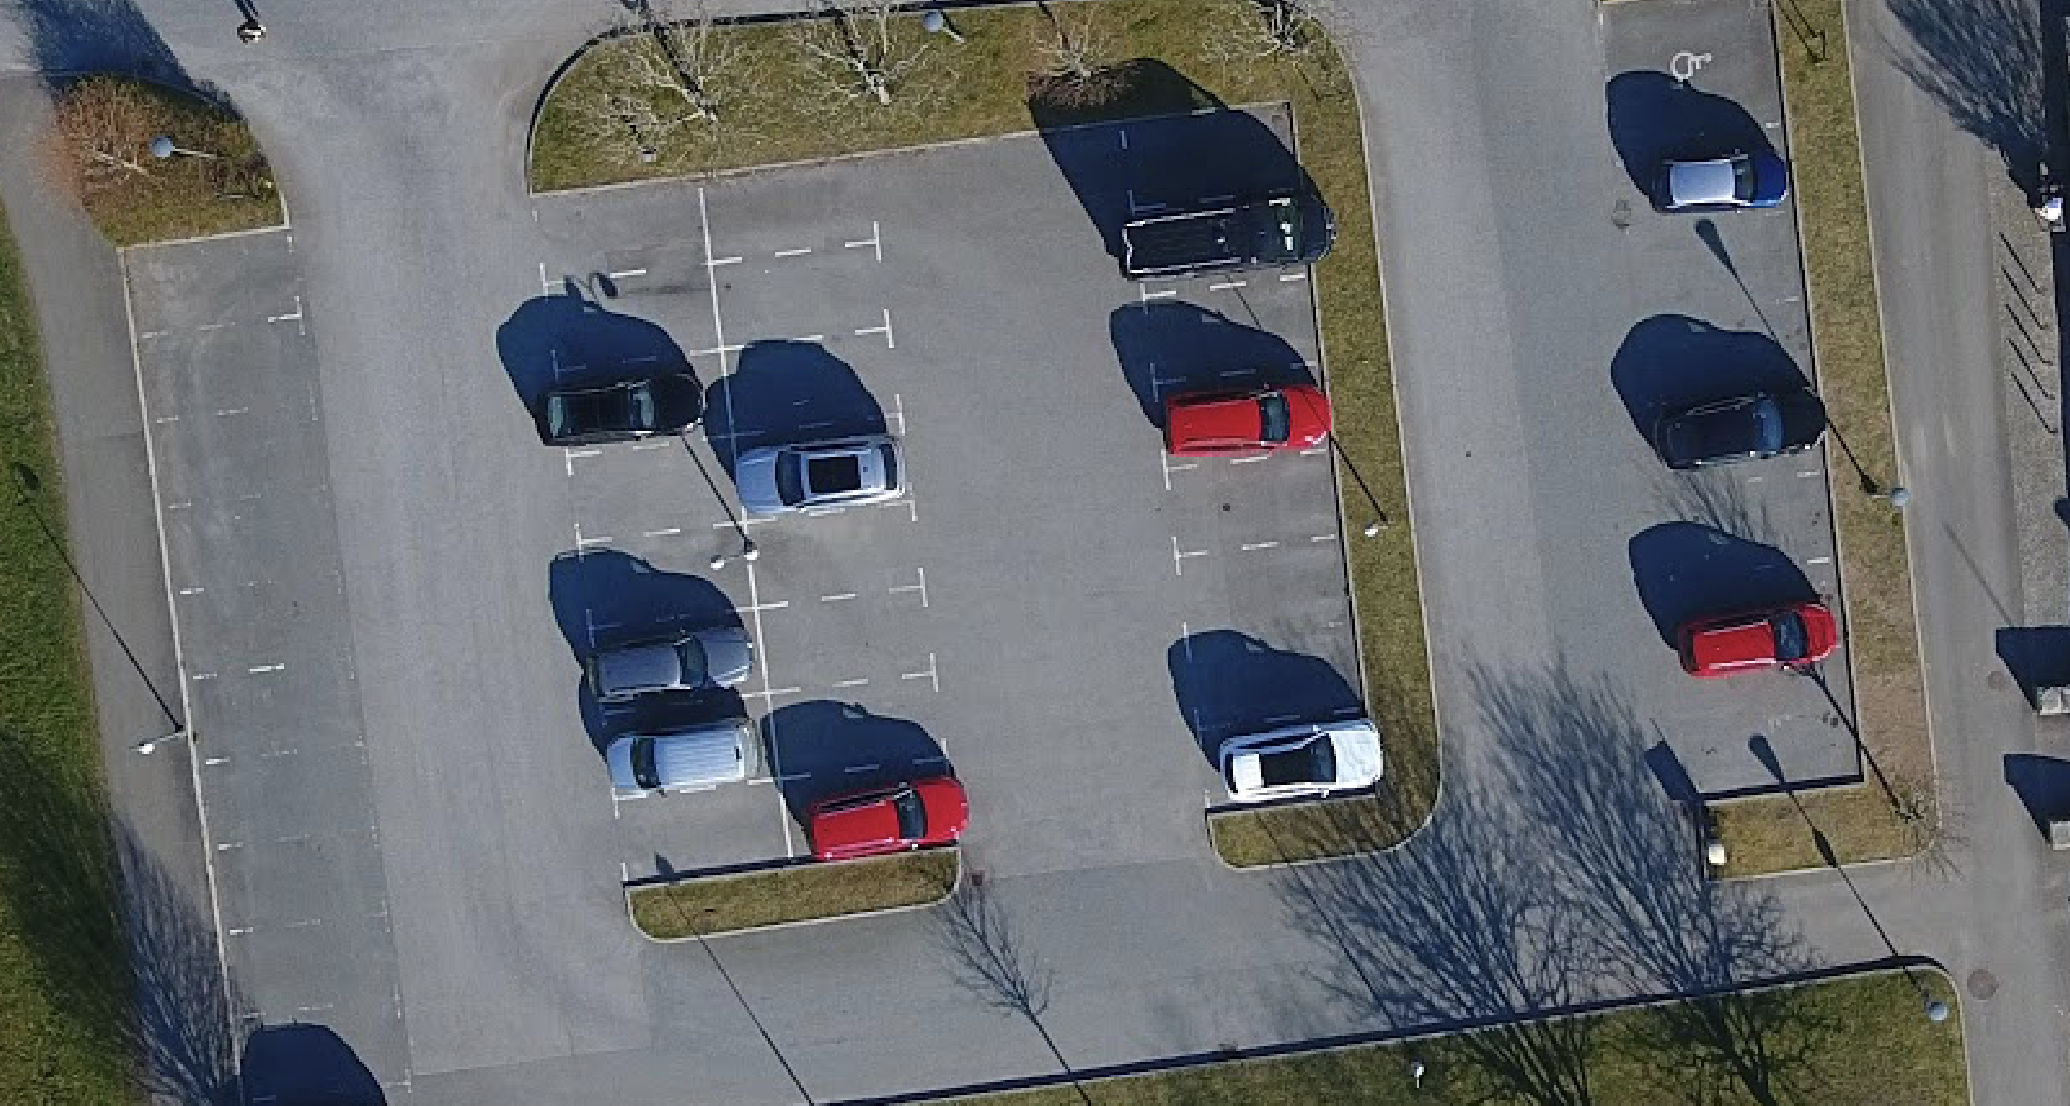
\includegraphics[width=\textwidth]{figure/parking1}}
  \end{subfigure}
  \quad
  \begin{subfigure}[b]{0.395\textwidth}
    \frame{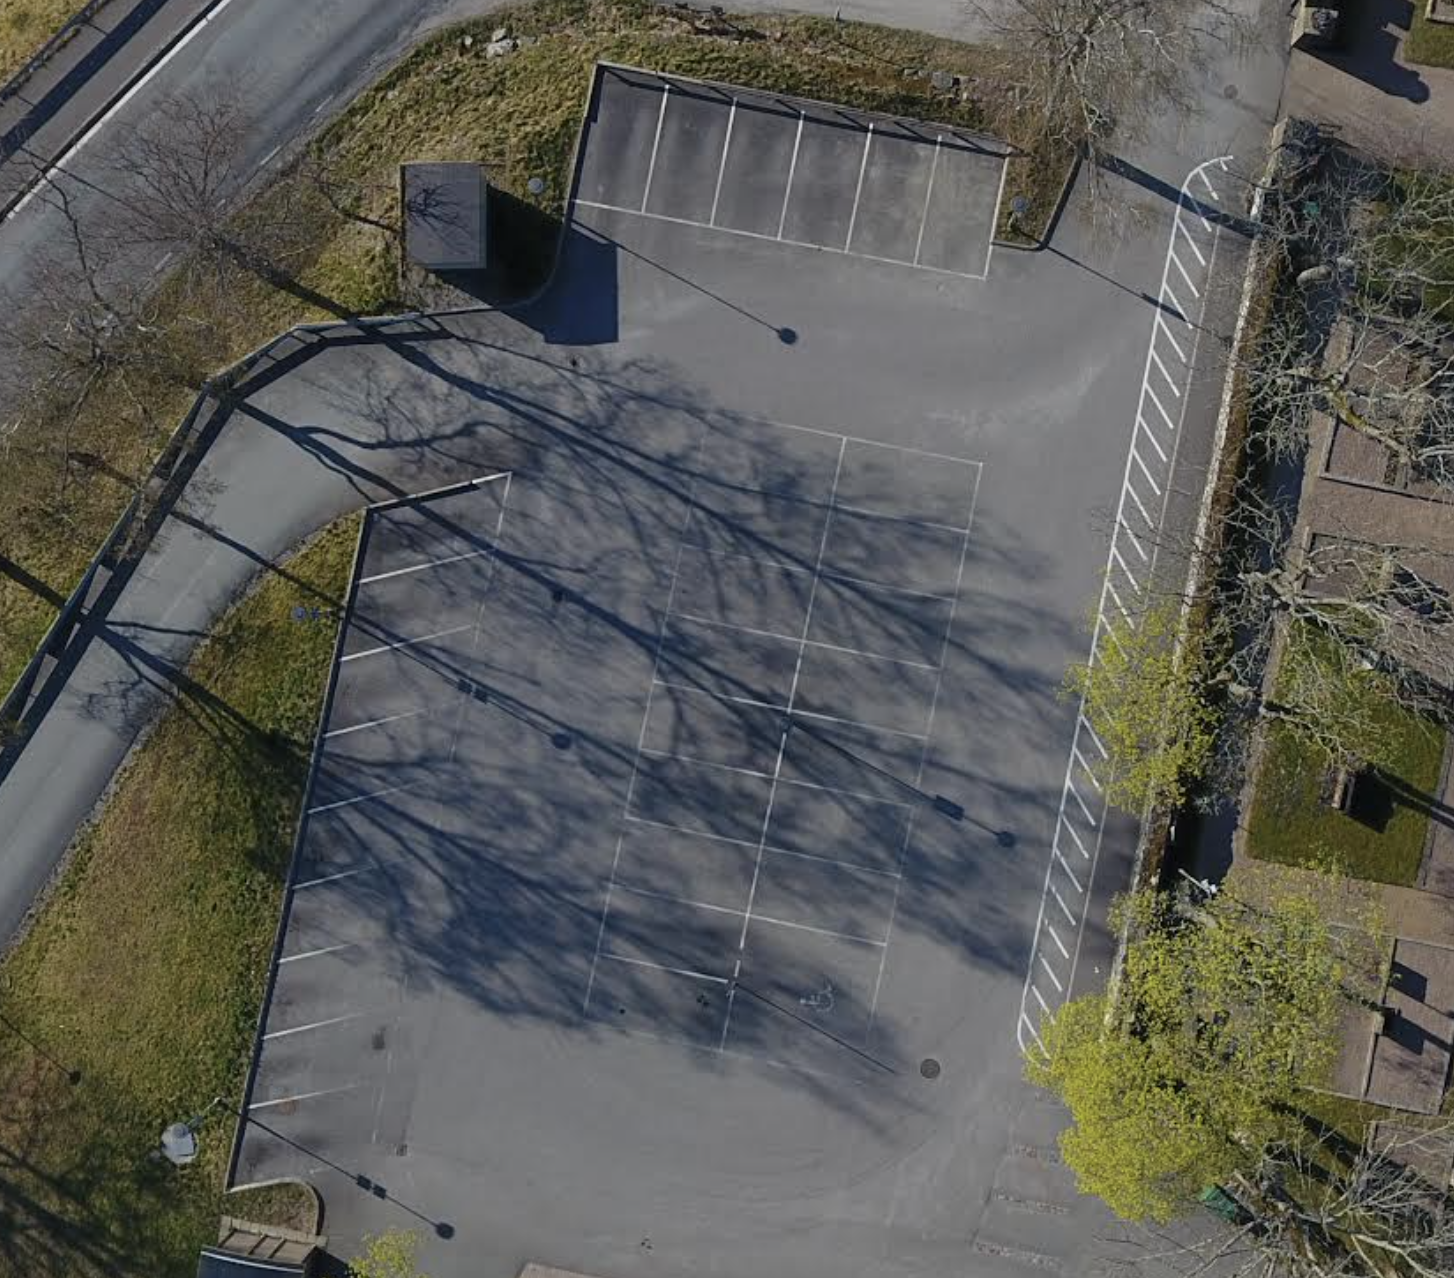
\includegraphics[width=\textwidth]{figure/parking2}}
  \end{subfigure}

  \caption{Two examples of parking lots observed by the project group, showcasing the rectangular shapes mentioned above.}
  \label{fig:parkings}
\end{figure}
Afterwards, based on the size of the rectangle, the algorithm would then generate either two, or four columns of parking spaces (see Figure~\ref{sizebased}.
